% Created 2025-02-04 Tue 21:37
% Intended LaTeX compiler: pdflatex
\documentclass[11pt]{article}
\usepackage[utf8]{inputenc}
\usepackage[T1]{fontenc}
\usepackage{graphicx}
\usepackage{longtable}
\usepackage{wrapfig}
\usepackage{rotating}
\usepackage[normalem]{ulem}
\usepackage{amsmath}
\usepackage{amssymb}
\usepackage{capt-of}
\usepackage{hyperref}
\usepackage{minted}
\author{Ross Mikulskis}
\date{\today}
\title{RT USB Streaming Protocol}
\hypersetup{
 pdfauthor={Ross Mikulskis},
 pdftitle={RT USB Streaming Protocol},
 pdfkeywords={},
 pdfsubject={},
 pdfcreator={Emacs 29.4 (Org mode 9.8-pre)}, 
 pdflang={English}}
\begin{document}

\maketitle
\tableofcontents

\section{Introduction}
\label{sec:orga16d977}
Quest is a Real-Time Operating System (RTOS) that supports scheduling tasks
in an isolated, predictable manner. We've developed RT-DDS, a
publisher-subscriber framework which connects services over shared
memory communication channels in pipelines to ensure end-to-end
latency, throughput, and loss requirements. Each service in RT-DDS is
a tuned-pipe with an input and output endpoint and thread bound to a
VCPU (Virtual CPU) with a corresponding budget \(C\) and period \(T\)
using rate-monotonic scheduling (RMS).

Similarly, we can schedule USB bandwidth reservations with a budget
and period over isochronous endpoints for real-time USB
communication. Currently Quest only supports bulk transfer endpoints,
and these endpoints cannot be scheduled for real-time
transactions. Therefore, bulk transfers may be stalled on account of
pending isochronous requests on the host, which may be on other USB
lines.

Using xDCI (Extensible Device Controller Interface) drivers, we can
emulate a device over USB using a gadget driver, for example Linux
supports Ethernet over USB from host to host.
\section{Project goal}
\label{sec:org3aa0e6f}
We want to finish the implementation of the xDCI driver on Quest to support
isochronous endpoint communication. Using the xDCI driver, we plan to write a
real-time USB gadget device driver with our own custom protocol. We can then
extend RT-DDS for cross-host pipelines. See the image below which depicts
two hosts communicating over an isocrhonous USB endpoint.
\begin{center}
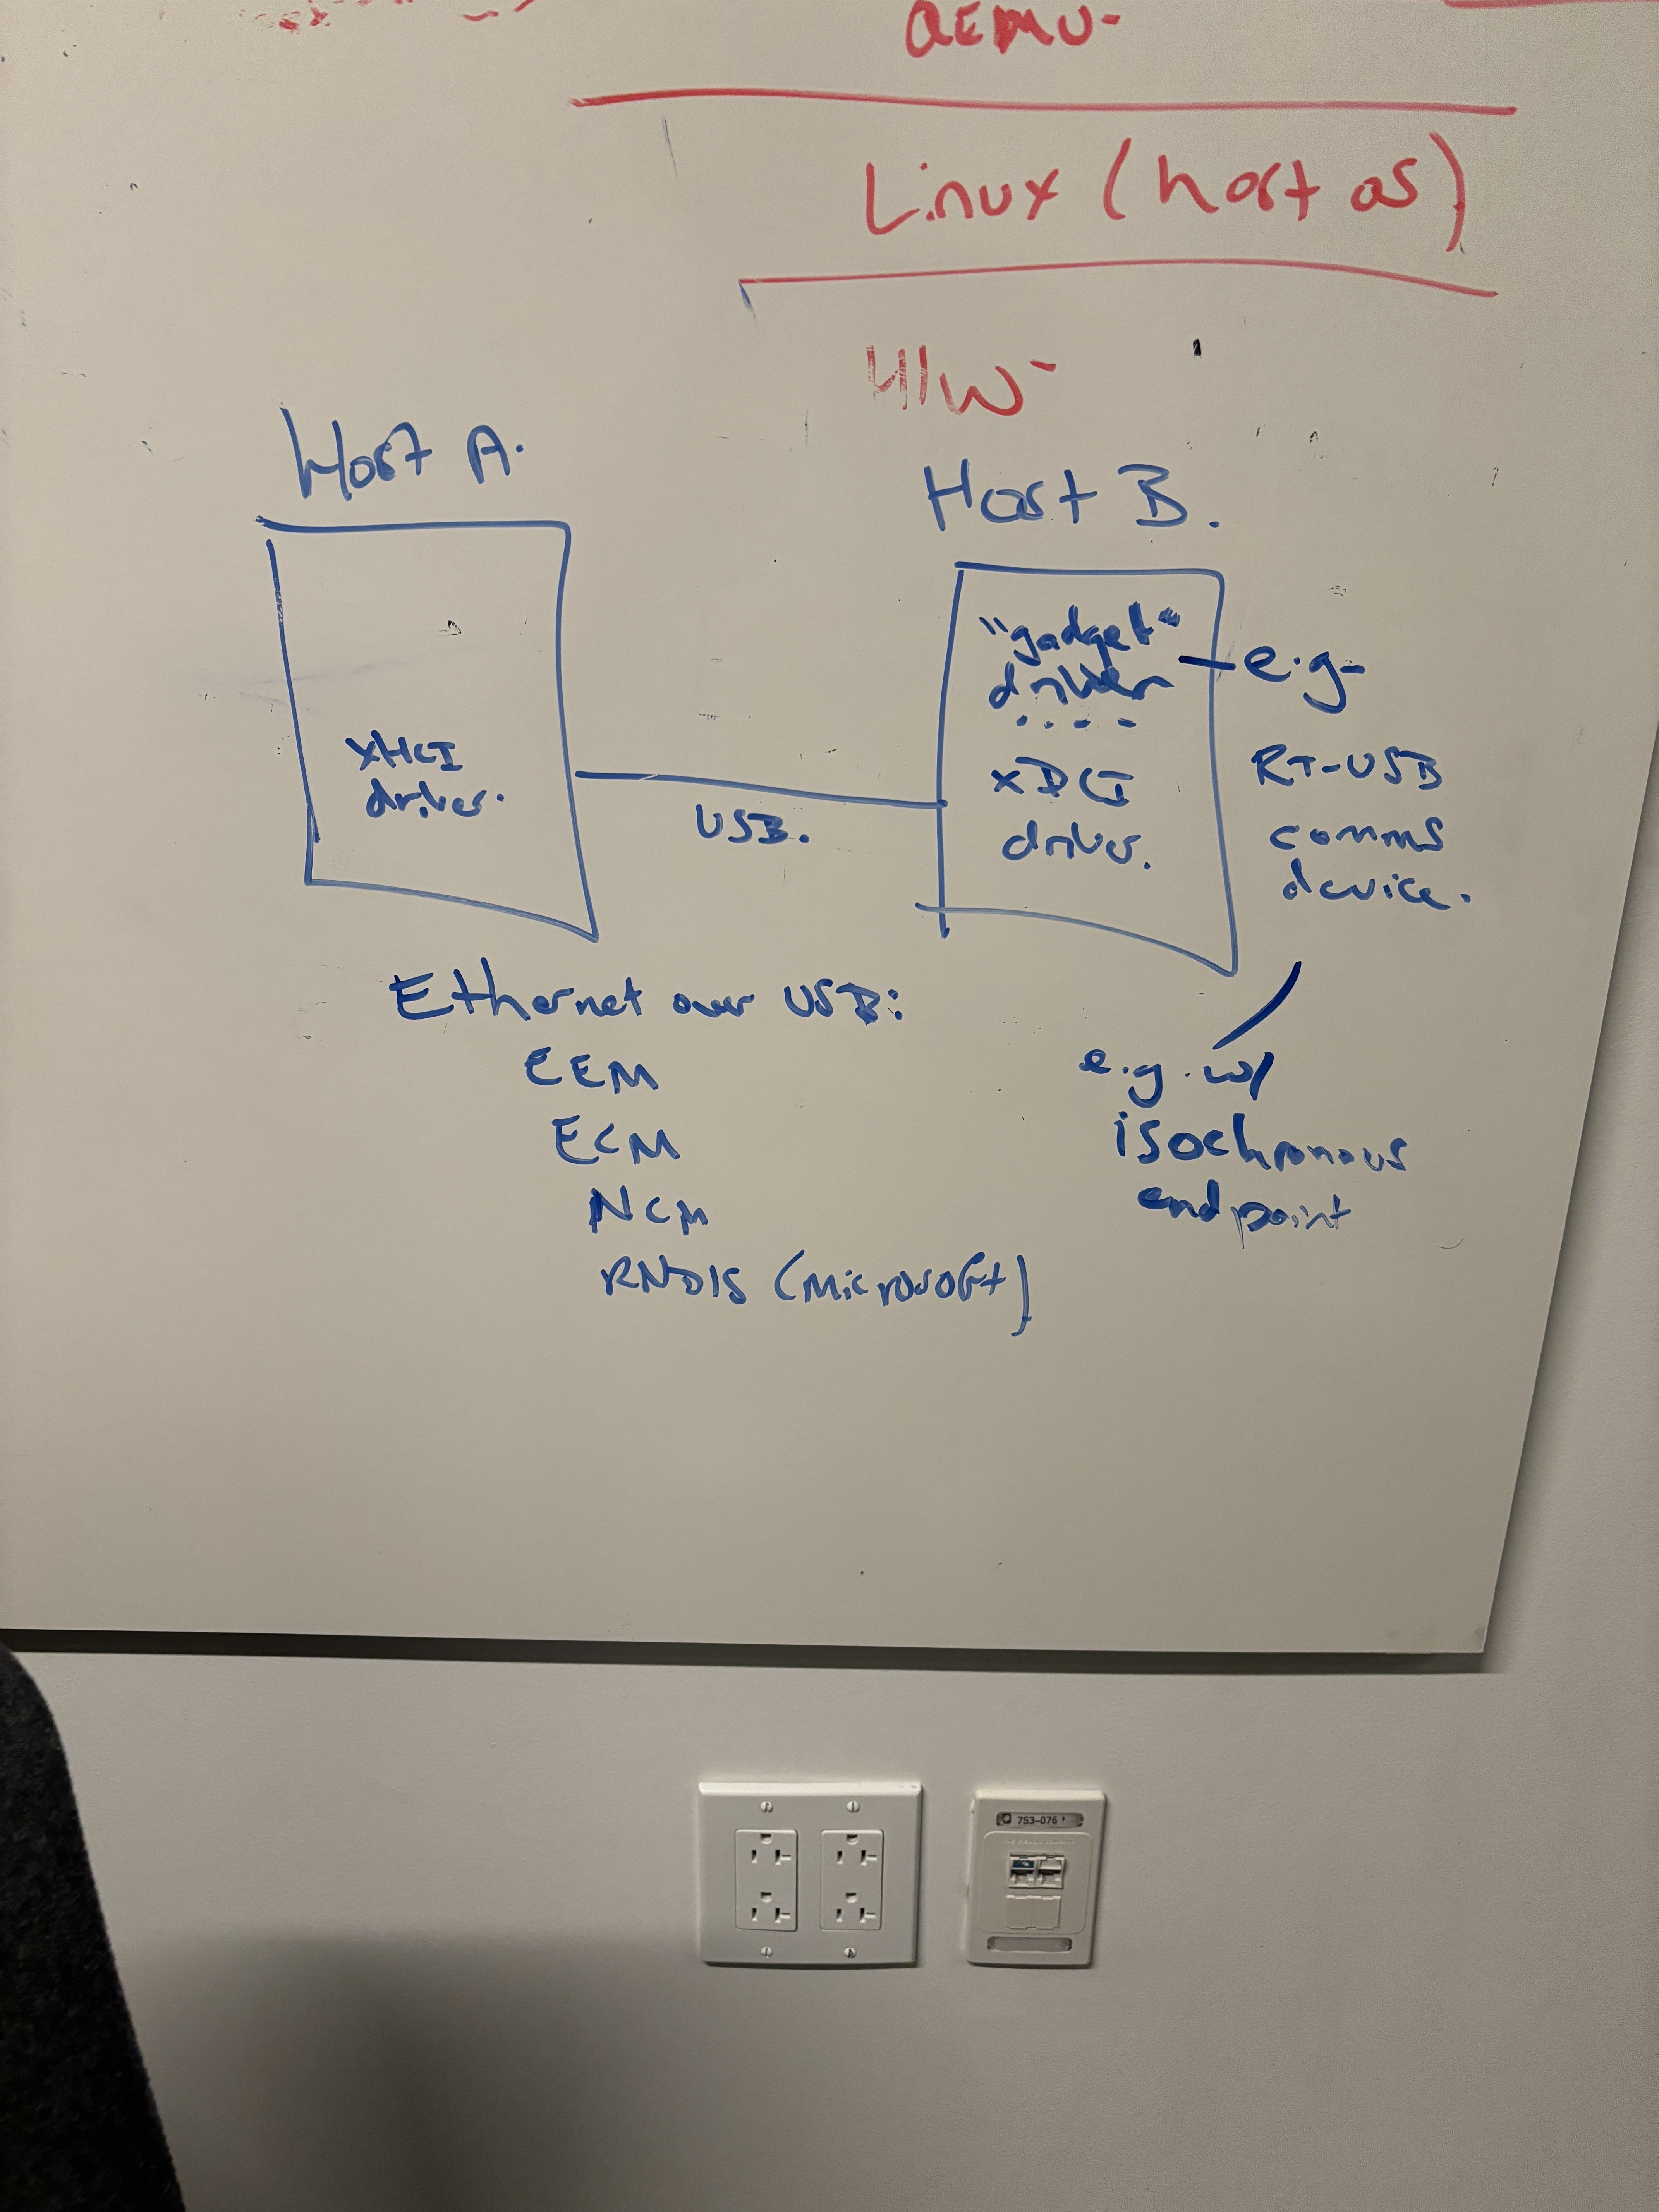
\includegraphics[width=.9\linewidth]{./rt-usb.JPG}
\end{center}
\section{Tasks to complete}
\label{sec:org736c52a}
\begin{enumerate}
\item finish implementation of the xDCI driver on Quest and
\item develop a RT-USB gadget device driver to support isochronous endpoints
on Quest
\item (reach goal) support RT-DDS pipelines spanning hosts over USB using this
RT-USB gadget device driver
\begin{itemize}
\item Incorporate USB latency calculations in RT-DDS scheduler
\end{itemize}
\end{enumerate}
\section{Required skill set}
\label{sec:org374e33a}
\begin{itemize}
\item Knowledge of xDCI USB spec
\item Embedded systems programming skills, C coding
\end{itemize}
\section{Resources}
\label{sec:orgd2f4bcf}
\href{https://www.cs.bu.edu/\~richwest/papers/rtas2024-final-revised.pdf}{USB Interrupt Differentiated Service for Bandwidth and Delay-Constrained Input/Output}
\end{document}
